Figure \vref{fig:svsitesting} presents the evolution of the fitness function ($TOTFIT$) against the number of ants in the colony (swarm size), in the case of four routes. The algorithm is run one time for each swarm size, and the $TOTFIT$ value is recorded for each iteration. In the first iteration, all edge values are zero, and the first point in the graph represents the $TOTFIT$ value after the first iteration. Figure \vref{fig:svsiruntime} presents the time it takes in seconds to run 100 iterations for each swarm size. 

As one can observe in Figure \vref{fig:svsitesting}, increasing the size of the colony leads to a better $TOTFIT$ value in both the initial and final iterations. However, increasing the swarm size, these values seems to converge at approximately the same value for all cases.

As one can see in Figure \vref{fig:svsiruntime}, when $s$ increases from 100 to 125, the runtime increases close to exponentially, compared to a close to linear growth from 25 to 100.

Because of this, and because of the small difference between the swarm size of 100 and 125, the selected value for $s$ is 100. All values seems to converge after around 40 iterations, and to be sure, the selected value for $i$ is 50.

\begin{figure}[H]
\begin{center}
  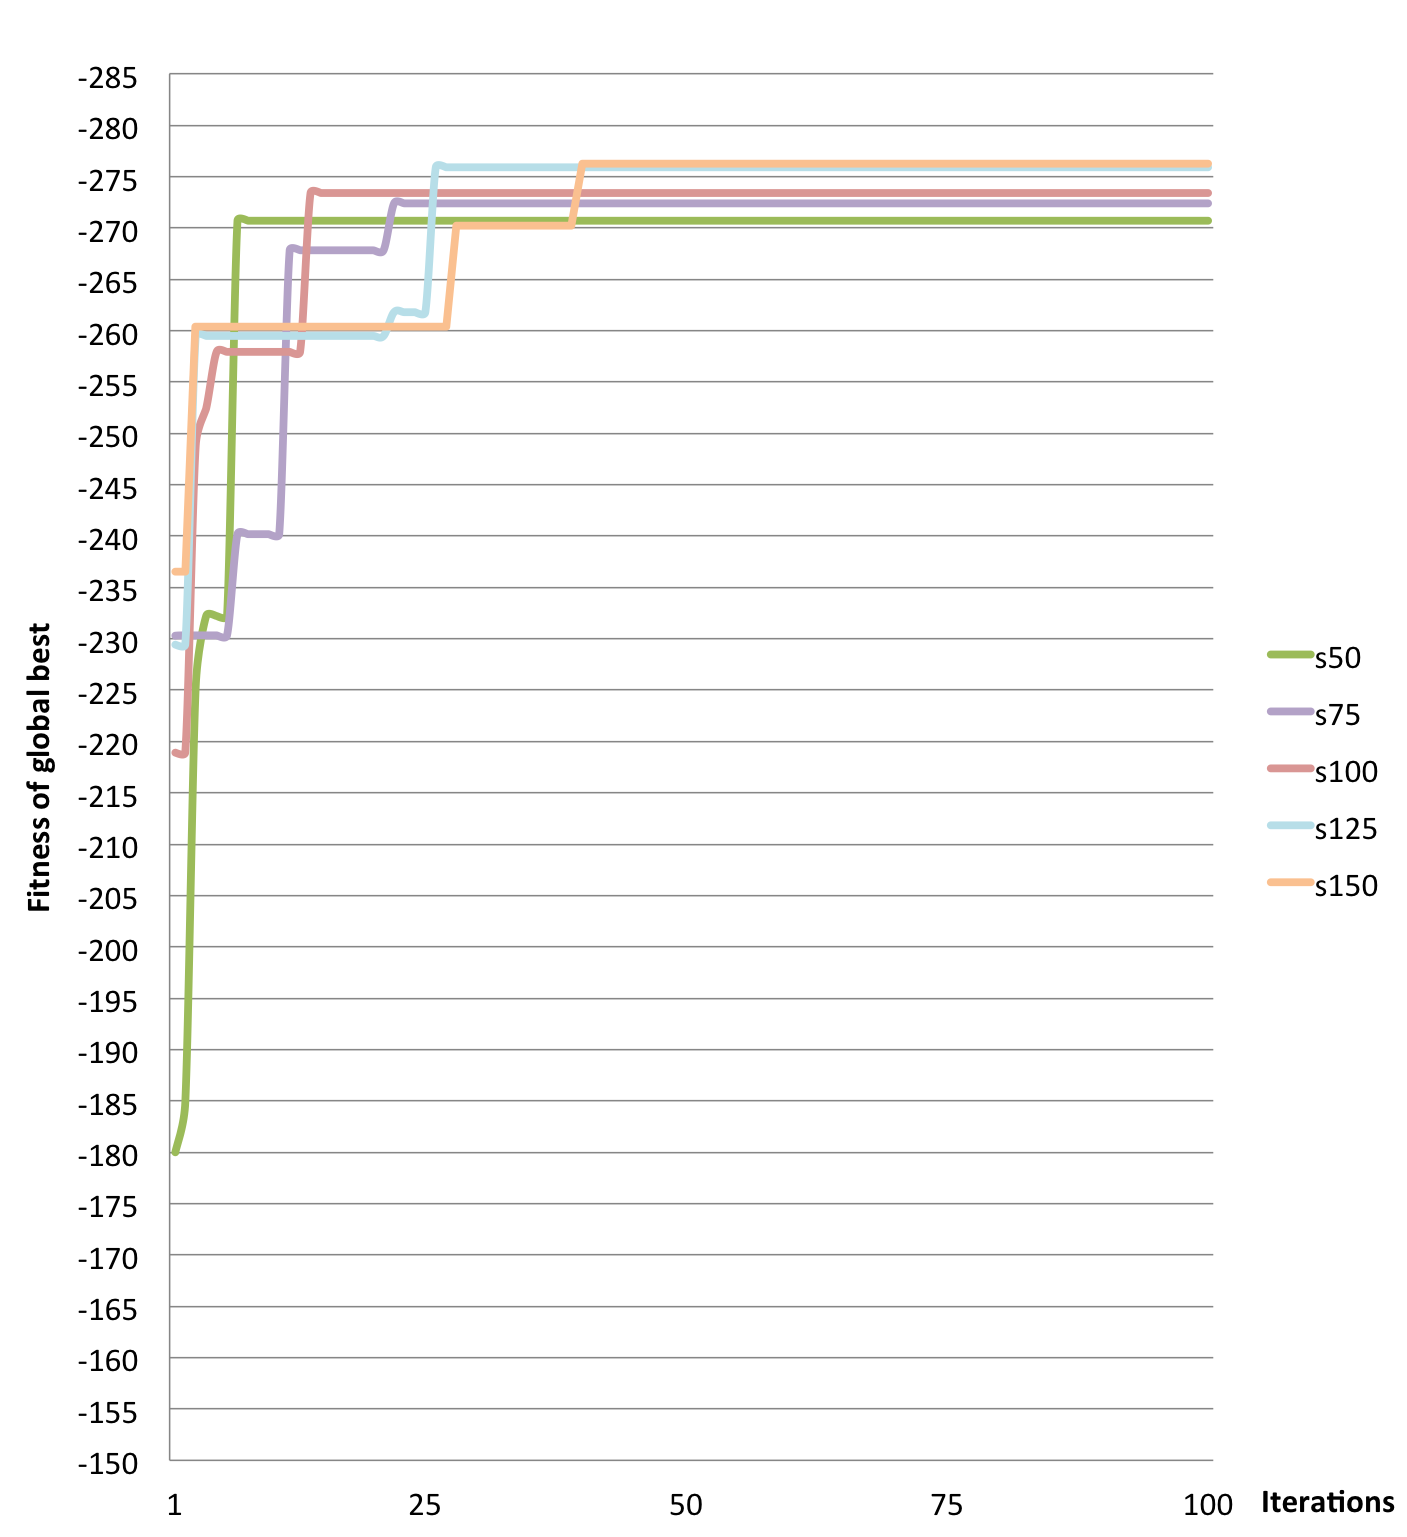
\includegraphics[width=4in]{assets/svsitest.png}
  \end{center}
  \caption{Evolution of total fitness function against the number of ants in the swarm (s)}
  \label{fig:svsitesting} 
\end{figure}

\begin{figure}[H]
\begin{center}
  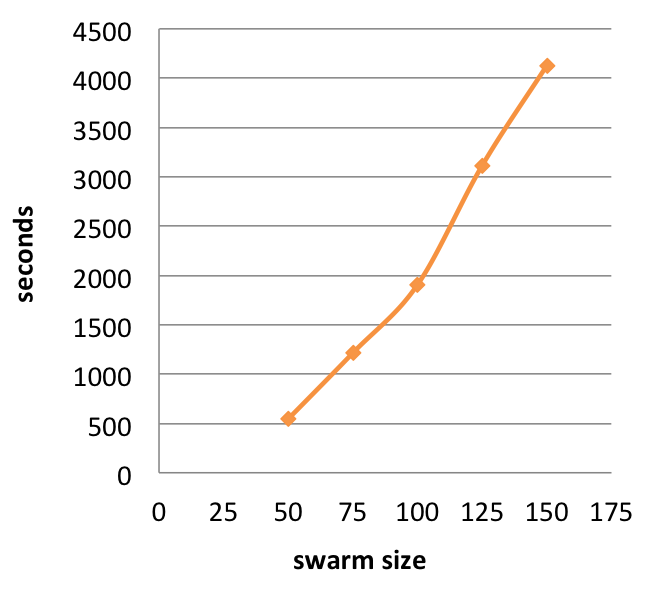
\includegraphics[width=2.5in]{assets/svsiruntime.png}
  \end{center}
  \caption{Evolution of the runtime, in seconds, in accordance to the swarm size}
  \label{fig:svsiruntime} 
\end{figure}
